\documentclass[11pt]{article}
\usepackage{graphicx}

\begin{document}
\title{Lesson 9}
\author{Colt Bradley}
\date{}
\maketitle

\section{Exercise 1}
For the first exercise, I take a simple Euler method solution to solve for radioactive decay. I then add a while loop which increases the time steps by a factor of 10 each time, save the error, and time steps into a file, then plot them on a log plot. 

\begin{figure}[ht]
\centering
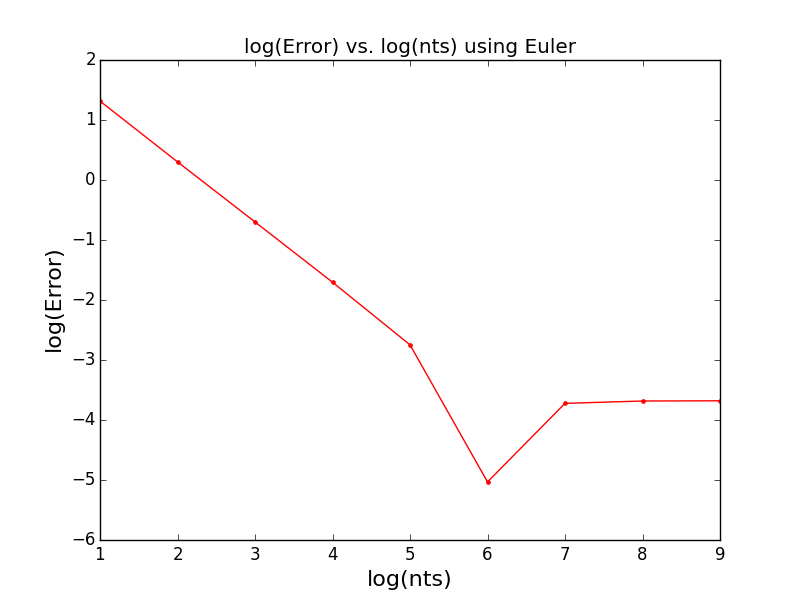
\includegraphics[scale=.5]{eulererrorplot.png}
\caption{Log plot for the error using Euler method to solve differential equations }
\end{figure}

The plot is linear, implying the error goes as $\delta t$ as expected from the derivation. In the next section, we`ll compare this to the Runge-Kutta method.
 
\section{Exercise 2}
The Runge-Kutta method is a two step process that goes proportional to $\delta t^2$. We'll preform the same analysis as we did for the Euler method, and the relationship between time steps and error shouldn't be linear, as we see below. 

\begin{figure}[ht]
\centering
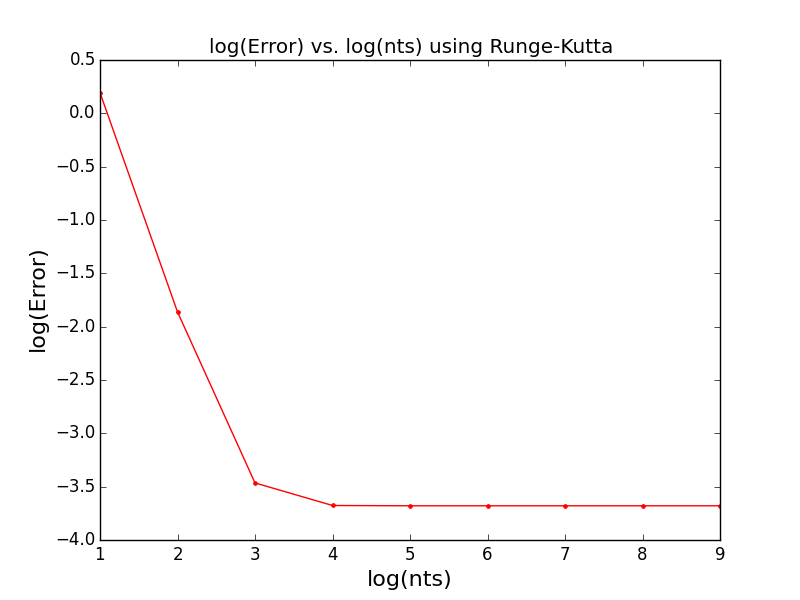
\includegraphics[scale=.5]{rkerrorplot.png}
\caption{Log plot for the error using Second order Runge-Kutta method to solve differential equations. When the line flattens, it is because we have hit the limit for computer memory.  }
\end{figure}

Comparing the Euler and Runge-Kutta method for 100 time steps, we see that the error for the Euler method is $2.00\%$, compared to $.014\%$ for the Runge-Kutta method. For the Euler method to yeild a comparable error, we have to go to 10,000 time steps. 


\section{Code}

\begin{verbatim}
#Colt Bradley
#2.9.16
#Homework 9

#import numpy and pylab
import numpy as n
import pylab as p

###################################################
#Exercise 1
###################################################

#define values
n0 = 100
tau = 5.
tf = 10.
ts = 10
dt = tf/ts
i = 0.
data = []
error = []
nts = []

#for Loop
while ts < 10000000000: 
    n0 = 100
    i=0
    dt = tf/ts  
    while i < ts: 
        n0 = n0 - n0*dt/tau
        i = i+1
    nts.append(ts)
    ts = ts*10
    err = (13.5335-n0)/13.5335*100
    err = abs(err) 
    data.append(n0)
    error.append(err)

#write answer to file
n.savetxt("eulerdata.txt", zip(nts,data,error))

#read back the data, plot in Log plot
X,Y = n.loadtxt("eulerdata.txt",usecols = (0,2), unpack = True)
X = n.log10(X)
Y = n.log10(Y)
p.close()
p.plot(X,Y,"r")
p.plot(X,Y,"r.")
p.title("log(Error) vs. log(nts) using Euler")
p.xlabel("log(nts)",fontsize=16)
p.ylabel("log(Error)", fontsize=16)
p.show()
p.savefig("eulererrorplot.png")

#################################################
#################################################]
#Exercise 2
#################################################

#define values
n0 = 100
tau = 5.
tf = 10.
ts = 10
dt = tf/ts
i = 0.
data = []
error = []
nts = []

#for Loop
while ts < 10000000000: 
    n0 = 100
    i=0
    dt = tf/ts  
    while i < ts: 
        n1 = n0 - n0*dt/2/tau
        n0 = n0 - n1*dt/tau
        i = i+1
    nts.append(ts)
    ts = ts*10
    err = (13.5335-n0)/13.5335*100
    err = abs(err) 
    data.append(n0)
    error.append(err)

#write answer to file
n.savetxt("rkdata.txt", zip(nts,data,error))

#read back the data, plot in Log plot
X,Y = n.loadtxt("rkdata.txt",usecols = (0,2), unpack = True)
X = n.log10(X)
Y = n.log10(Y)
p.close()
p.plot(X,Y,"r")
p.plot(X,Y,"r.")
p.title("log(Error) vs. log(nts) using Runge-Kutta")
p.xlabel("log(nts)",fontsize=16)
p.ylabel("log(Error)", fontsize=16)
p.show()
p.savefig("rkerrorplot.png")
\end{verbatim}


\end{document}